\section{Layout}
The layout for this system is also done in Altium desginer and is attached in appendix C. The layout for TK510, TK511, TK520, TK530, TK531, and TK532 is completed, and attached. The source files in Altium format can be found at \citep{githubtesla}.

\subsection{PCB identification}
To easily identify the pcbs (and modules) markings are placed in silk screen of all the pcbs in the same way. The Part number of the module, the date manufactured. And Omega Verksteds logo. See \cref{fig:tk530_tekst}.
\begin{figure}
    \centering
    
\includegraphics[width=0.6\textwidth]{img/TK530_Tekst.PNG}
    \caption{Detail from TK530 PCB}
    \label{fig:tk530_tekst}
\end{figure}

\subsection{Power back plane (TK530)}
The stackup for the power back plane is two layers with no copper plane fill. Two layers is chosen because of the low complexity of the layout, and no copper plane fill is chosen to increase separation of low and high voltage signals. The traces for the HVDC supply voltage are drawn as thick as reasonable and the supply connections are placed in the middle between the two power amplifier modules. The connections for the output signal are placed as close to the card connectors as possible, and the solder mask on the trace from the power amplifier and the load capacitor is omitted so that additional solder may be added to the trace to increase the area of the trace. Warning labels are added next to all exposed metal with higher than 50V (peak) voltage. The width of the pcb is chosen from the price breaks of the pcb supplier. Card holders to add mechanical stability to the inserted modules are mounted directly to the pcb, these guide the modules and ensures the module mates correctly with the connector. Some mechanical fastening to the chassis should also be used to fix the module in place. The thickness of the substrate was chosen to be 3mm to increase the mechanical strength.


\subsection{Signal back plane}
The connectors for the power modules are offset to prevent power modules to be inserted in signal module slots and vice versa. The same card holders as used on the power back plane are used on the signal back plane. The width of the signal back plane is chosen from the price breaks of the pcb supplier.


\subsubsection{Signal module form factor}
The width of the signal module is given by the width of the signal back plane minus the space used for the card holders. The height is chosen from the height of the card holders, and the closest price break of the pcb supplier. The form factor chosen is shown in \cref{fig:tk511_img}
\begin{figure}
    \centering
    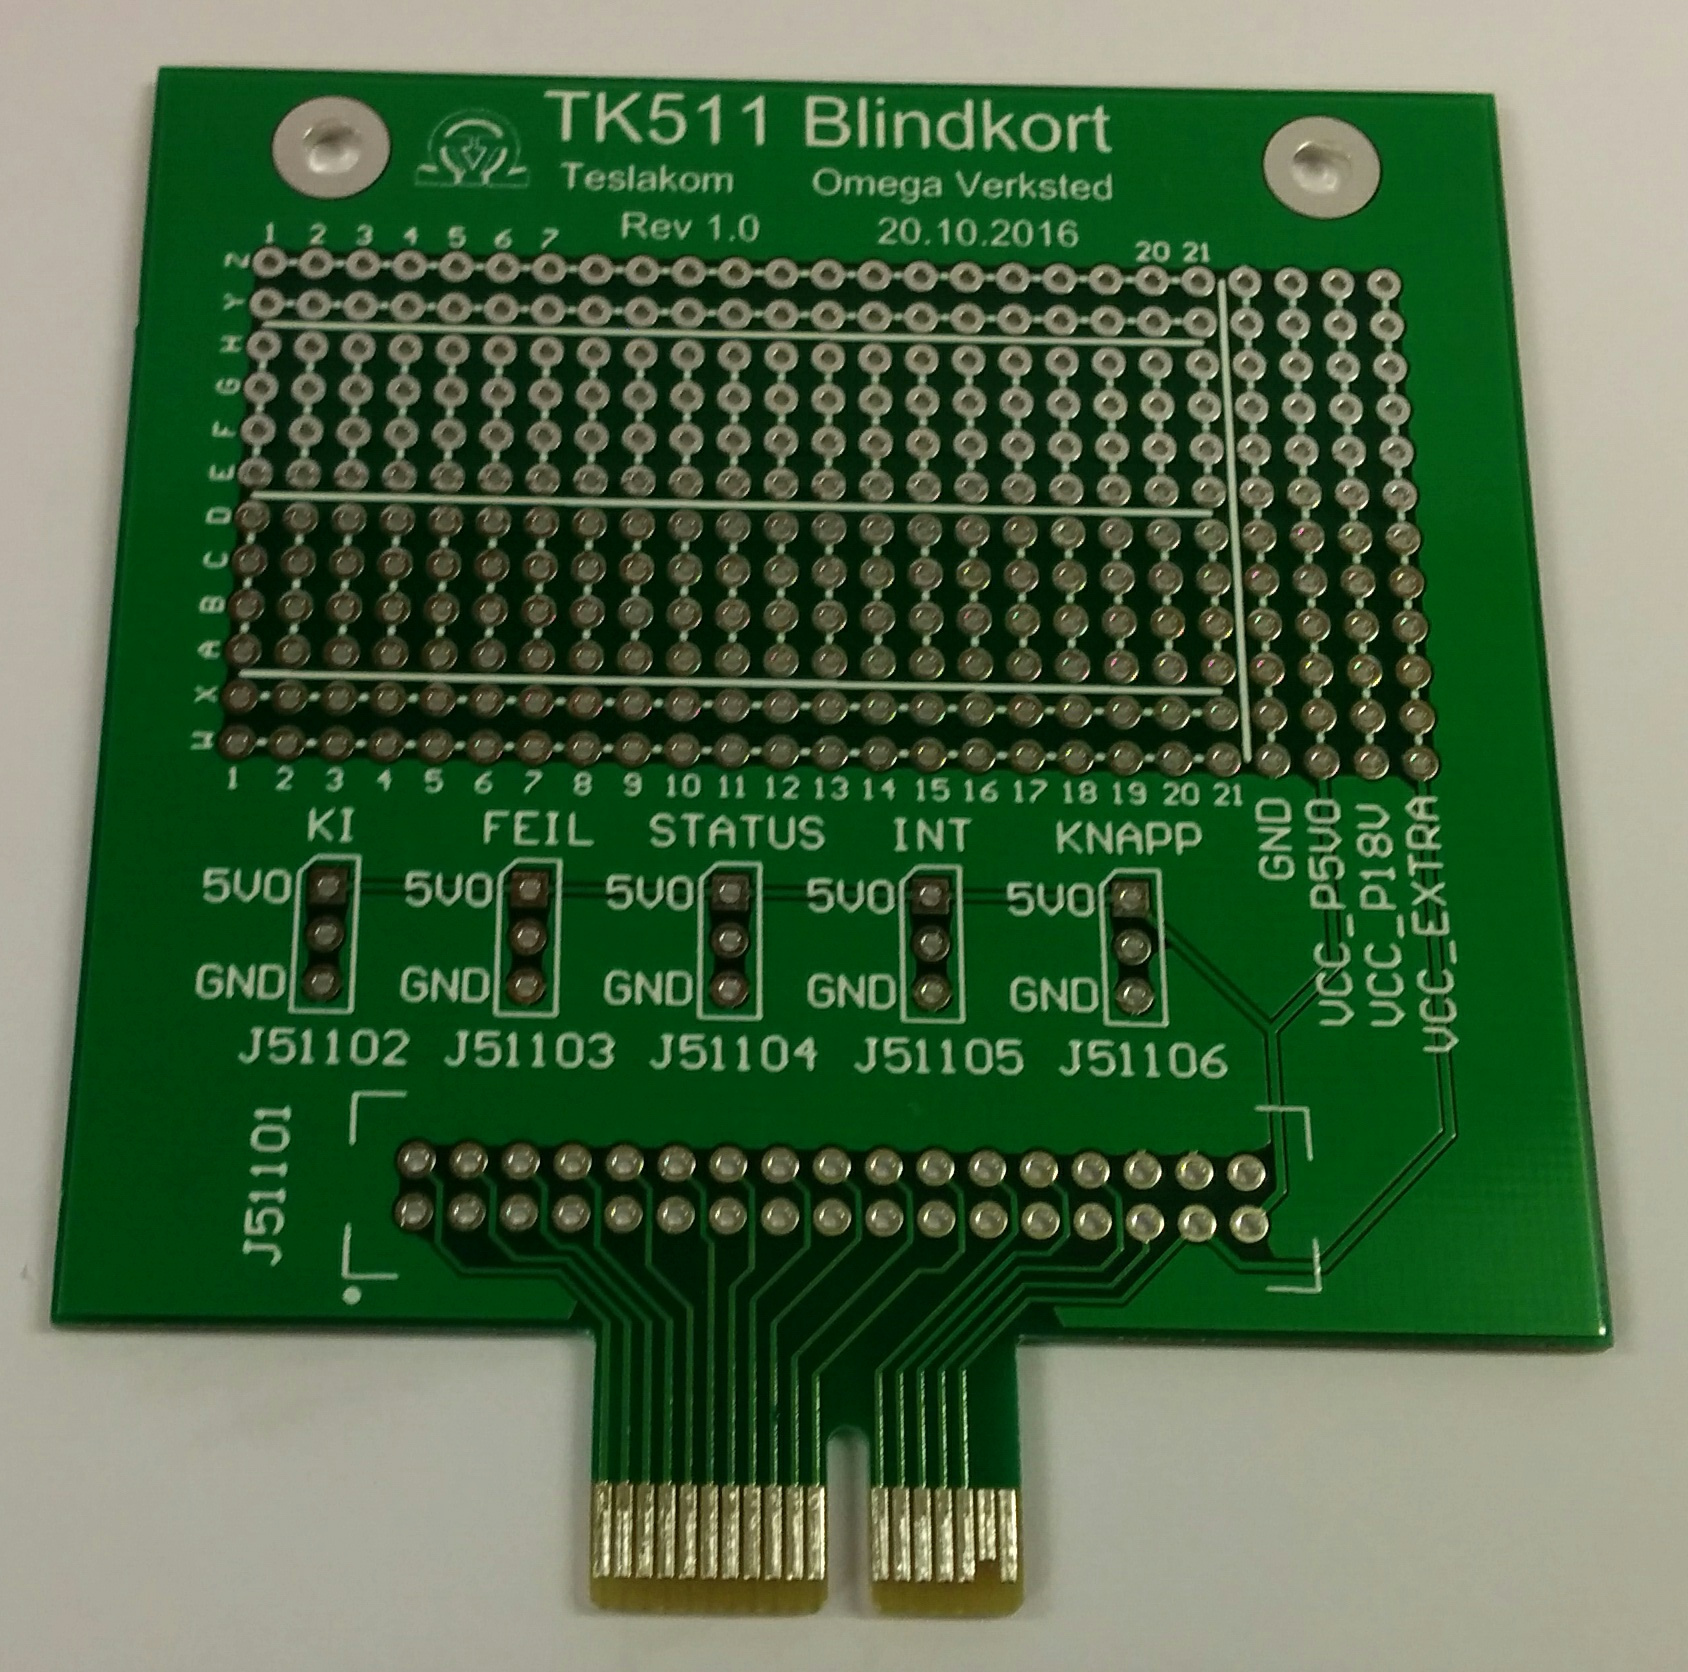
\includegraphics[width=0.5\textwidth]{img/TK511_Blindkort.jpg}
    \caption{Signal module pcb}
    \label{fig:tk511_img}
\end{figure}

\subsubsection{Power supply module form factor}
The form factor for the power supply modules is the same as for the signal modules with the exception of the connector being offset.

\subsubsection{Power module form factor}
For the power modules back plane connectors from samtec with four powerful pins and 16 signal pins was chosen. The width is chosen as the same as the signal modules.
The form facor chosen is shown in \cref{fig:TK531}.
\begin{figure}
    \centering
    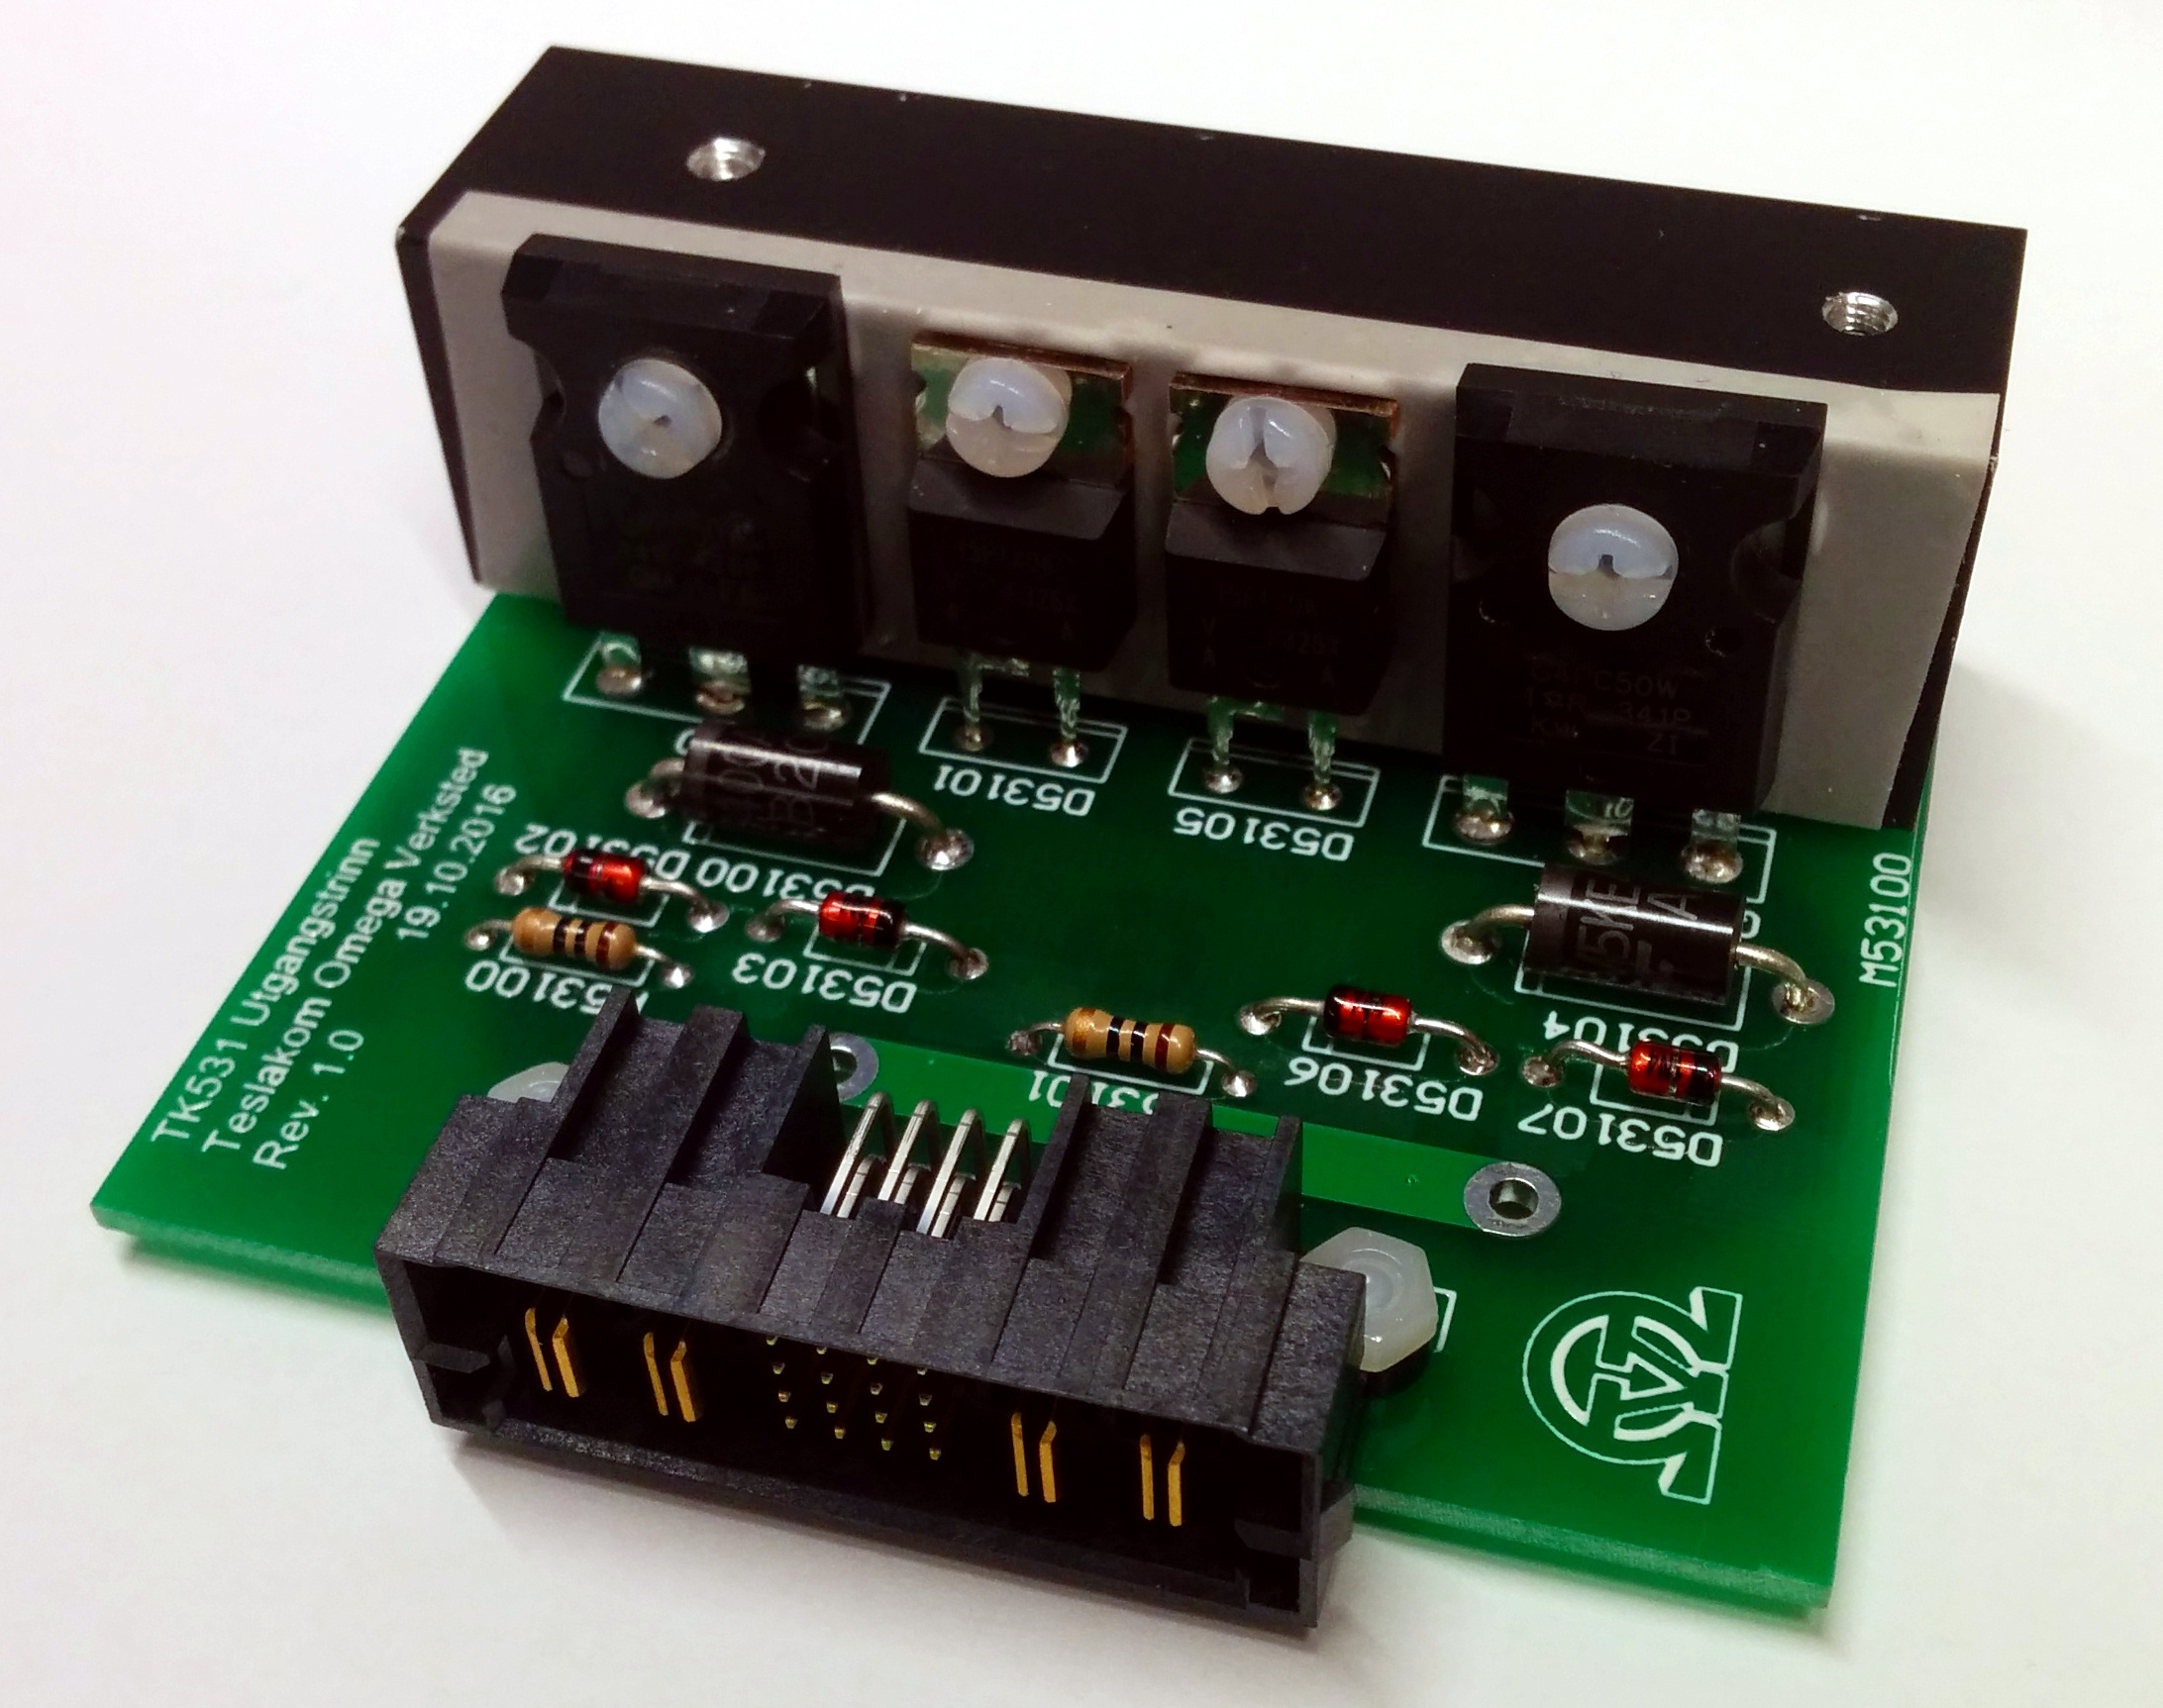
\includegraphics[width=0.5\textwidth]{img/TK531_IMG.jpg}
    \caption{Power module form factor}
    \label{fig:TK531}
\end{figure}